% With Plot %
\documentclass[12pt]{article}
\usepackage{pgf,tikz,pgfplots}
\pgfplotsset{compat=1.12}
\usepackage{mathrsfs}
\usetikzlibrary{arrows}
\pagestyle{empty}
\begin{document}
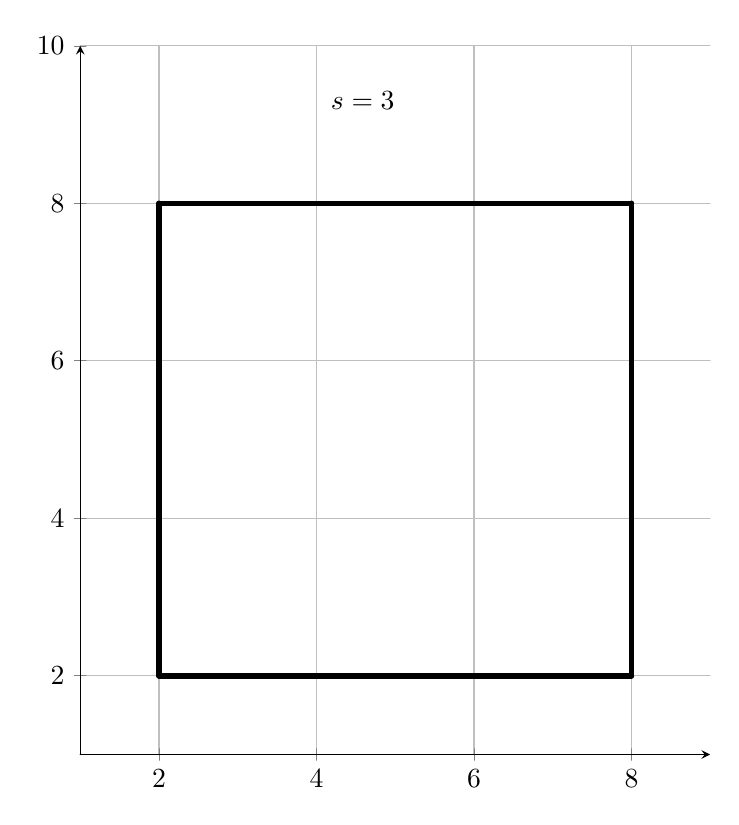
\begin{tikzpicture}[line cap=round,line join=round,>=triangle 45,x=1.0cm,y=1.0cm]
\begin{axis}[
x=1.0cm,y=1.0cm,
axis lines=middle,
ymajorgrids=true,
xmajorgrids=true,
xmin=1.0,
xmax=9.0,
ymin=1.0,
ymax=10.0,
xtick={2.0,4.0,...,8.0},
ytick={2.0,4.0,...,10.0},]
\clip(1.,1.) rectangle (9.,10.);
\draw (4.0586054744228335,9.543745809905824) node[anchor=north west] {$s = 3$};
\draw [line width=2.pt] (2.,8.)-- (8.,8.);
\draw [line width=2.pt] (8.,8.)-- (8.,2.);
\draw [line width=2.pt] (8.,2.)-- (2.,2.);
\draw [line width=2.pt] (2.,2.)-- (2.,8.);
\end{axis}
\end{tikzpicture}
\end{document}
% END With Plot %

% Without Plot %
% \documentclass[10pt]{article}
% \usepackage{pgf,tikz}
% \usepackage{mathrsfs}
% \usetikzlibrary{arrows}
% \pagestyle{empty}
% \begin{document}
% \begin{minipage}{\linewidth}
%   \begin{center}
%     \begin{tikzpicture}[line cap=round,line join=round,>=triangle 45,x=1.0cm,y=1.0cm]
%       \clip(5.9,5.9) rectangle (9.1,9.6);
%       \draw [line width=2.pt] (6.,9.)-- (9.,9.);
%       \draw [line width=2.pt] (9.,9.)-- (9.,6.);
%       \draw [line width=2.pt] (9.,6.)-- (6.,6.);
%       \draw [line width=2.pt] (6.,6.)-- (6.,9.);
%       \draw (7.092938170839365,9.72892993303502) node[anchor=north west] {$s = 3$};
%     \end{tikzpicture}
%   \end{center}
% \end{minipage}
% \end{document}
% END Without Plot %
